\documentclass[10.5pt,onecolumn,a4paper]{article}%pre,aps,
\usepackage{ctex}
\usepackage{setspace,dcolumn}
\usepackage{graphicx}
\usepackage{float,psfrag,epsfig}
\usepackage{hyperref}
%\usepackage[font=small,format=plain,labelfont=bf,textfont=it,justification=raggedright,singlelinecheck=false]{caption}
\usepackage{enumerate}
\usepackage{amsmath}
\usepackage{longtable,tabularx,multirow}
\hypersetup{colorlinks=true}
\usepackage{geometry}
\geometry{top=2.54cm,bottom=2.54cm,left=3cm,right=3cm}
\usepackage{subcaption}
\usepackage{caption}
\usepackage{booktabs}%excel2latex
\usepackage{multirow}
\usepackage{multicol}
\usepackage{colortbl}%表格背景色
\usepackage{listings,xcolor}
\usepackage{array}
\usepackage{framed}
\lstset{frame=shadowbox,rulesepcolor=\color{red!20!green!20!blue!20}, %边框阴影
        numbers=left, %设置行号位置
        numberstyle=\tiny, %设置行号大小
        basicstyle=\tiny, %代码字体大小设定
        keywordstyle=\color{blue}, %设置关键字颜色
        commentstyle=\color[cmyk]{1,0,1,0}, %设置注释颜色
        %frame=single, %设置边框格式
        escapeinside=``, %逃逸字符(1左面的键),用于显示中文
        breaklines, %自动折行
        extendedchars=false, %解决代码跨页时,章节标题,页眉等汉字不显示的问题
        xleftmargin=2em,xrightmargin=2em, aboveskip=1em, %设置边距
        tabsize=4, %设置tab空格数
        showspaces=false %不显示空格
       }
   
\makeatletter
\def\verbatim{\scriptsize\@verbatim \frenchspacing\@vobeyspaces \@xverbatim}
\makeatother
   
   \renewcommand{\abstractname}{\LARGE Summary}

\title{美国FOF市场总资产的时间序列分析}
\author{祁周, 王喆, 任庆杰}

\begin{document}

\begin{titlepage}	
	\begin{center}	
		\includegraphics[width=0.2\textwidth]{./pkulogo}\\[1cm]    
		
		\textsc{\LARGE Peking University}\\[1.5cm]
		
		\textsc{\Large }\\[2cm]
		
		
		% Title

		{ \huge \bfseries FOF基金时间序列分析}\\[3cm]

		
		% Author and supervisor
		\begin{minipage}{0.4\textwidth}
			\begin{flushleft} \large
				\emph{\Large 作者:}\\
				\Large 祁周\\
				\Large 王喆\\
				\Large 任庆杰
			\end{flushleft}
		\end{minipage}
		\begin{minipage}{0.4\textwidth}
			\begin{flushright} \large
				\emph{\Large 指导老师:} \\
		\Large 涂云东
			\end{flushright}
		\end{minipage}
		
		\vfill
		
		% Bottom of the page
		{\large \today}
		
	\end{center}
	
\end{titlepage}






\include{abstract}
\clearpage

\section{引言}
基金中基金(fund of funds,简称FOF)是指投资于其他基金组合的基金.在欧美市场,基金中基金已经发展成为数量和规模均较大的一类成熟的理财产品.在美国市场上, FOF市场总资产在1995年初仅有3891.54百万美元,到2016年底已发展为1439637.04百万美元,年均增长率高达30.84\%.

2016年9月,中国证券监督管理委员会发布《公开募集证券投资基金运作指引第2号------基金中基金指引》,标志着公募基金行业迎来创新品种FOF,并由此进入FOF发展的全新时代.
\subsection{基金中基金的起源}

基金中基金起源于上世纪70年代,最初是以其他私募股权基金(private equity fund)为投资的标的.这是因为私募股权基金往往设置有非常高的投资门槛,单笔投资的资金规模巨大,并且要求参与者为合格投资者,这使得许多有意愿投资私募股权基金的个人投资者被拒之门外.而PE FOF作为渠道,解决了这个问题,使得个人投资者可以通过投资PE FOF,即间接地投资一篮子私募股权基金,来分享风险投资可能带来的高收益.

与中国市场不同,美国法律对于没有明确规定禁止的事情,默认为许可,而在中国,公民仅能做法律允许的事.这使得美国资本市场的创新能力非常强大,非常有利于全新产品的创立.

\subsection{基金中基金的成熟契机}

1987年10月19日,美国股票市场在经历了两年的牛市之后,遭受到一次巨大的股灾,这也是历史上继1929年经济危机后第二次全球经济危机.道琼斯指数单日跌幅达22\%,恒生指数暴跌11\%,这促使投资者开始思考如何根据市场的不同情况配置不同种类的基金,分散标的,减小风险.

\begin{figure}[ht]
\begin{minipage}[ht]{0.47\textwidth}
\centering
\includegraphics[width=\textwidth]{pic/mutual.pdf}
\subcaption{}\label{fg:mutual}
\end{minipage}%
\hspace{0.06\textwidth}
\begin{minipage}[ht]{0.47\textwidth}
\centering
\includegraphics[width=\textwidth]{pic/retirement.pdf}
\subcaption{}\label{fg:retirement}
\end{minipage}
\caption{美国FOF基金相关市场发展:(a)1988--2016年美国股票、共同基金市场发展状况;(b)1974--2016年美国退休养老资产发展状况}
\end{figure}

共同基金在这次惨重的股灾过后,也不断开发出新的产品,基金的类型迅速增多,整个基金市场呈现爆发式增长,如图~\ref{fg:mutual}~所示,基金数量甚至远超股票数量.市场的复杂性、基金的多样性使得投资者对基金筛选及风险分散有了极大的需求,从此, FOF市场规模的扩大有了客观上的推动因素.

在同一时期,美国也大规模推广401(k)计划,这个计划的主要内容是创建了一个税收优惠账户,对雇员和雇主共同缴纳的养老金进行投资过程中收取的股息税和资本利得税进行减免.这为随后养老金进入资本市场打开了通道.

\subsection{基金中基金与养老金的关系\label{sec:retire}}

如上文所述,退休养老资产的扩大成为了美国基金中基金市场规模扩大的重要因素.为了能够吸引养老金投资者,基金公司推出了大量的针对养老金需求的基金中基金产品. 尽管FOF具有双重收费的劣势, 但它双重风险分散、多样化投资的优势吸引了大量养老金投资者的青睐.

退休养老基金主要投资于基金中基金产品,而基金中基金市场的主要资金来源也是退休养老基金,二者相互依存.基金中基金解决了养老金投资的难点,将两者紧密联系在一起.

\subsection{美国FOF市场的总资产序列}
根据彭博资讯提供的数据可以获取美国市场上所有FOF基金的规模及成立时间,以此统计出全市场的数量和规模,如图~\ref{fg:fof}~所示,时间区间为1995年1月至2017年5月,具体数据如表~\ref{tab:fof}~所示.
\begin{figure}[ht]
  \centering
  \includegraphics[width=0.6\textwidth]{pic/fof.pdf}
  \caption{1995年以来美国基金中基金市场的数量及规模}\label{fg:fof}
\end{figure}

如图~\ref{fg:fof}~所示,美国基金中基金市场的资产规模呈上升趋势,显示出明显的时间趋势.

\textcolor{red}{补充:把之前proposal中的数据描述,翻译成汉语,稍作修改,补充在这个地方,by王喆}

\textcolor{red}{修改:这部分引言是我自己写的,请二位提一提意见,然后我来修改,修改意见请二位单独写一个文件,或者像我一样加入红色的说明,否则的话容易被覆盖掉,by王喆\& RQJ}



\section{美国FOF市场总资产}
\subsection{ARIMA建模}
首先使用ADF检验, 在备择假设为平稳性的条件下, 对FOF基金的资产总量数据进行检验. 检验结果为$P=0.8158$, 这说明FOF的资产总量数据并不是一个平稳的时间序列. 而对FOF资产总量取对数差分后,即得到总资产的对数增长率序列${GR\_ast_t}$, 再次进行ADF检验, 检验结果$P<0.01$, 拒绝了非平稳的原假设, 即其对数差分后是一个平稳序列.

\textcolor{red}{展示: AST和GR\_ast的ADF检验结果, by王喆. }

下面对对数差分后的序列进行ARMA建模. 绘制$GR\_ast_t$的自相关和偏自相关图像可以发现, 此序列的ACF函数在5阶处截尾, PACF函数在5阶处结尾. \emph{经过反复尝试,} 当使用MA(5)对序列进行刻画时, 可以得到较好的估计效果. MA(5)模型的极大似然估计结果如下:

\textcolor{red}{展示: 定阶所用的数据或其图示, by王喆}

\textcolor{red}{展示: MA(5)的极大似然估计结果的表格或图示, by王喆}

\subsection{模型诊断}

对估计的残差$\hat{u}_t$进行Ljung-Box检验, $p=0.84$, 可以接受原假设, 满足白噪声要求. 同时绘制$\hat{u}_t$的自相关函数, 从1阶开始都不显著, 也说明$\hat{u}_t$序列不存在自相关.

\textcolor{red}{展示: 残差的白噪声检验结果及其ACF、PACF图示, by王喆}

继续对$\hat{u}_t^2$进行 McLeod.Li检验, 判断是否存在ARCH效应. 检验结果各阶的$P$值都接近1, 说明不存在ARCH效应.

\textcolor{red}{残差平方的第一次检验结果或其图示, by王喆}

但是, 如果绘制出标准化的残差图进行观察, 会发现在第90期有一个明显的异常值. 很有可能因为这个异常值的出现, 使得其他的波动被隐藏, 在模型诊断的检验中造成了偏差. 通过Bonferroni法则进行检验MA(5)模型, 在第90期存在一个强影响点$GR\_ast_{90}$. 这进一步确认了我们的猜测.

\textcolor{red}{在上一段补充: Bonferroni法则的简要介绍, 用几句话说一下就好, by王喆}

\textcolor{red}{展示: 异常值的图示\&各种诊断情况, by王喆}

\subsection{异常值处理}
为了削弱第90期的异常值对模型的影响, 令
$$GR\_ast_{90} = \frac{1}{3} \cdot (GR\_ast_{89}+GR\_ast_{90}+GR\_ast_{91})$$
重新对${GR\_ast_t}$序列进行建模估计.
此时对使用极大似然估计得到的残差序列${\hat{u}_t^2}$进行 McLeod.Li检验, 检验结果$P$值很小, 拒绝了不存在条件异方差的原假设, 即存在GARCH效应. 于是使用 ARMA(0,5)-GARCH(0,1) 对调整后的${GR\_ast_{t}}$进行建模. 估计结果如下:

\textcolor{red}{写出模型的完整表达式,展示每个参数的值和标准差,by王喆}

\textcolor{red}{展示: 最新模型的预测结果,就是beamer里面的那一堆图,by王喆}

\textcolor{red}{修改: 统一一下上面几段用到的ARCH和GARCH字样,by王喆}


\section{美国养老金资产建模}
美国养老金市场资产中的IRA与DC计划部分是积极投资类型的,FOF市场的一大部分投资来源于这两部分养老金资产.所以我们着重研究养老金中IRA与DC计划这两部分资产和的时间序列.由于数据的局限性,我们只搜集到2007-2016年的季度数据,07年之前只搜集到年度数据.
\begin{figure}[h!]
	\begin{minipage}[ht]{0.47\textwidth}
		\centering
		\includegraphics[width=1\textwidth]{pic/re/niandu}
		\subcaption{}\label{niandu}
	\end{minipage}%
	\hspace{0.06\textwidth}
	\begin{minipage}[ht]{0.47\textwidth}
		\centering
		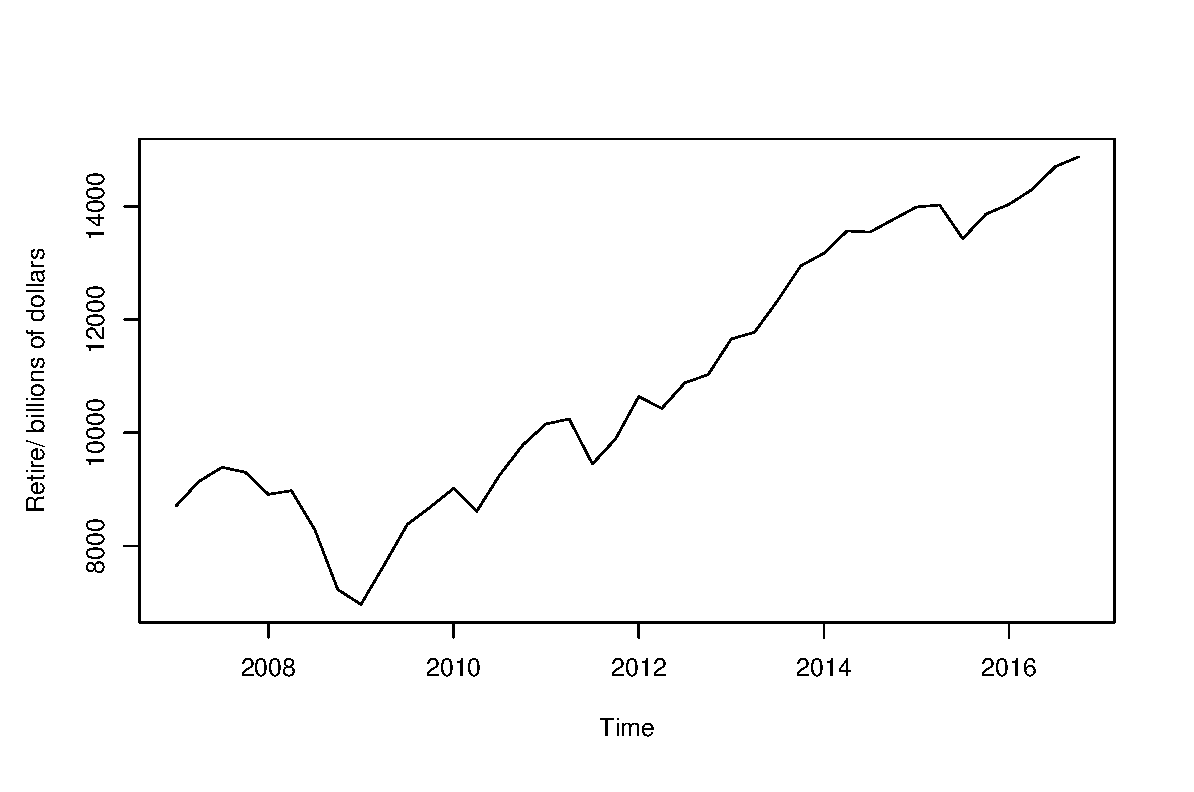
\includegraphics[width=1\textwidth]{pic/re/jidu}
		\subcaption{}\label{jidu}
	\end{minipage}
	\caption{美国养老金资产,IRA+DC部分:(a)1974-2016年IRA+DC年度数据;(b)2007-2016年IRA+DC季度数据}\label{reshuju}
\end{figure}
见图\ref{reshuju},分别是养老金中IRA+DC部分的1974-2016年度数据与2007-2016季度数据.可以看到,序列在2000年之前的波动比较小,在很长一段时间都处于缓慢增长阶段,这与近10年来的情况显著不同,即07年之后的季度数据更具有分析价值.综合考虑,我们采取2007-2016年的季度数据进行建模分析.
\subsection{白噪声序列}
\begin{figure}[h!]
	\centering
	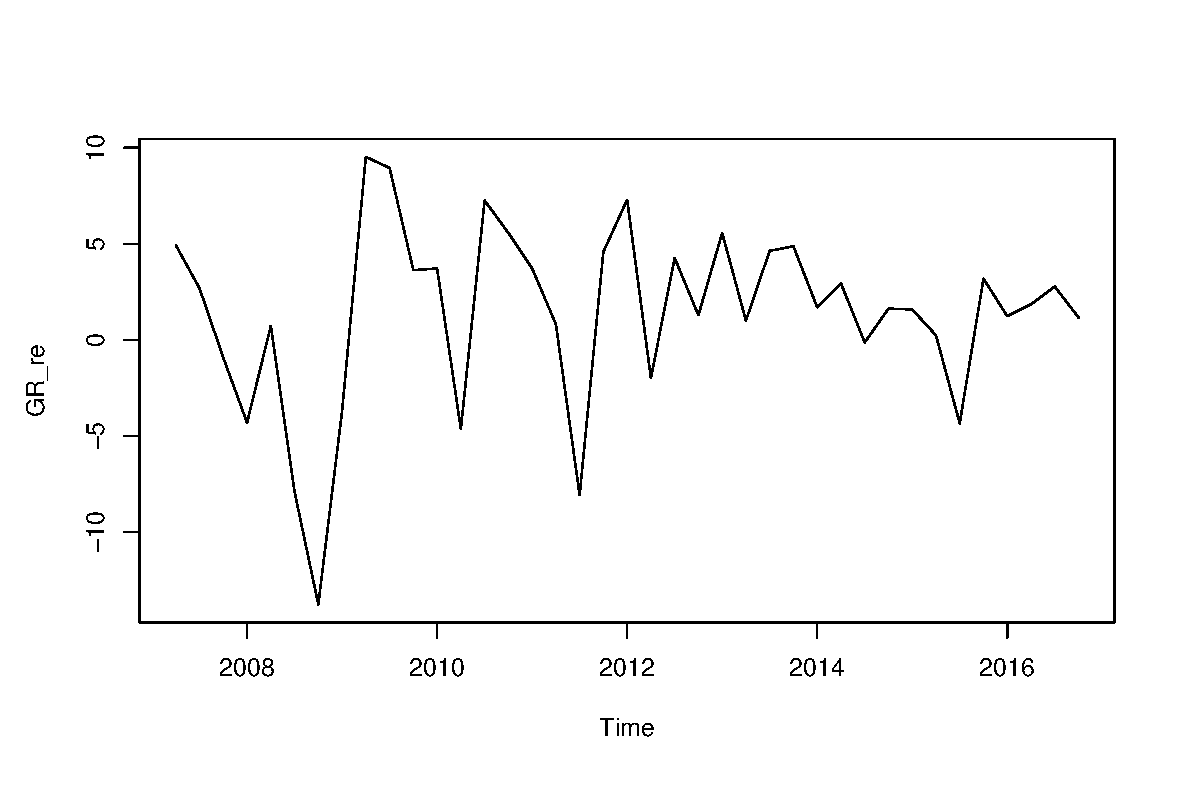
\includegraphics[width=0.5\linewidth]{pic/re/grre}
	\caption{美国养老金资产中IRA+DC部分的对数增长率序列}
	\label{fig:grre}
\end{figure}
如图\ref{fig:grre}所示,我们对上述的养老金季度数据序列进行了对数差分,得到了对数增长率序列.特别的,序列在08年之后出现了相当大的负向波动,这与08年的金融危机对应,由于DC计划可以提前取现,所以在金融危机发生时,发生了较大的资产流失.可以看出,序列大致是平稳的,这一点从ADF检验也可以看到.如下,其$p-value = 0.1231$,在85\%的置信度来说,我们应该拒绝原假设,即序列是平稳的.
\begin{framed}
	\begin{verbatim}
	 	Augmented Dickey-Fuller Test 
	 data:  GR_re
	 Dickey-Fuller = -3.1498, Lag order = 3, p-value = 0.1231
	 alternative hypothesis: stationary
	\end{verbatim}
\end{framed}
进一步,我们对序列进行一阶与二阶Ljung-Box检验,结果如下:
\begin{framed}
	\begin{verbatim}
 	Box-Ljung test                                                   Box-Ljung test
 data:  GR_re                                                       data:  GR_re^2
 X-squared = 14.69, df = 24, p-value = 0.9295              X-squared = 16.588, df = 24, p-value = 0.8657
	\end{verbatim}
\end{framed}
可以看到其一阶与二阶都不存在相关性,即我们可以认为是无异方差的白噪声序列.从McLeod.Li.test也可以看出,见图\ref{fig:mcre},序列不存在ARCH效应.
\begin{figure}[h!]
	\centering
	\includegraphics[width=0.5\linewidth]{pic/re/mcre}
	\caption{美国养老金资产中IRA+DC部分的对数增长率序列的McLeod.Li.test检验}
	\label{fig:mcre}
\end{figure}


\subsection{养老金对数增长率序列分布分析}
如前,对养老金对数增长率序列进行分析发现其为近似的白噪声序列,无ARCH效应,故可对该序列的分布进行分析.如图\ref{fig:qqre}所示,
\begin{figure}[h!]
\centering
\includegraphics[width=0.5\linewidth]{pic/re/qqre}
\caption{养老金对数增长率序列与正态分布比较的QQ图}
\label{fig:qqre}
\end{figure}
是养老金对数增长率序列与正态分布比较的QQ图,可以看出明显的厚尾分布,并且在负向的厚尾更严重,说明养老金市场资产对负面影响更加敏感.更加具体的还可以从如下的峰度、偏度、Shapiro检验和Jarque Bera检验进行分析.
\begin{framed}
	\begin{verbatim}
	kurtosis(GR_re)                                                   skewness(GR_re)
	1.173374                                                              -0.978918
	\end{verbatim}
\end{framed}
\begin{framed}
	\begin{verbatim}
	Shapiro-Wilk normality test                                           Jarque Bera Test
	data:  GR_re                                                                  data:  GR_re^2
	W = 0.93066, p-value = 0.01887                                   X-squared = 9.9001, df = 2, p-value = 0.007083
	\end{verbatim}
\end{framed}
其中峰度是减去正态峰度后的统计量,可以看到该序列具有一个正的峰度值,即厚尾.由Shapiro-Wilk与Jarque Bera检验也可以看到,都拒绝了原假设,即此序列不是正态分布.


\section{与退休养老资产的协整关系}
由于美国FOF基金的兴起, 主要源于养老金市场的发展. 美国雇员逐渐选择将养老金计划由DB(Defined Benefit) Plan转向DC(Defined Contribute) Plan, 增大了养老金投资着的投资需求. 而FOF基金作为一种收益稳定、风险二次分散的基金, 自然受到了这些被动投资者的青睐. 下面, 利用彭博数据库中FOF基金资产总量和养老金资产总量的季度数据, 对FOF基金市场与养老金市场进行协整分析. 在2007--2016十年中, 二者的绝对数量和增长率变化趋势如下:

% 两个市场的趋势图像
\includegraphics[width=0.4\textwidth]{pic/3-0-1.eps}
\includegraphics[width=0.4\textwidth]{pic/3-0-2.eps}

\textcolor{red}{修改:将图片按照引言里的格式插入,对照代码即可,可能会需要subfigure命令,可以参考tex源文件里下面隐藏着的被注释掉的代码,by RQJ}

%\begin{figure}[ht]
%  \centering
%  \subfigure[Small Box with a Long Caption]{
%    \label{fig:subfig:a} %% label for first subfigure
%    \includegraphics[width=1.0in]{pic1.eps}}
%  \hspace{1in}
%  \subfigure[Big Box]{
%    \label{fig:subfig:b} %% label for second subfigure
%    \includegraphics[width=1.5in]{pic.eps}}
%  \caption{Two Subfigures}
%  \label{fig:subfig} %% label for entire figure
%\end{figure}

% 单位根检验部分
对${FOF_t}$和${Retire_t}$序列分别进行单位根检验. ADF检验和Phillips–Perron的结果接受了原假设(单位根过程), 并且Kwiatkowski–Phillips–Schmidt–Shin检验结果拒绝了原假设(平稳过程). 因此可以认为${FOF_t}$和${Retire_t}$是非平稳序列.
继续对它们的差分序列${\Delta FOF_t}$和${\Delta Retire_t}$进行单位根检验, 得到的结果表明它们是平稳序列. 所以, ${FOF_t}$和${Retire_t}$分别是2个$I(1)$序列. 下面对这两个序列进行协整估计.

% 协整部分
首先, 使用最小二乘法估计如下方程:
$$FOF_t = \alpha + \beta \cdot Retire_t + \mu_t$$
得到$\alpha$和$\beta$的估计量$\hat{\alpha}$和$\hat{\beta}$. 估计结果如表~\ref{tab:coin-OLS-estimate}~所示.

% OLS回归结果表格
\begin{table}[ht]
    \centering
    \caption{OLS估计量}
    \label{tab:coin-OLS-estimate}
    \begin{tabular}{l | rrrr}
        Coefficients: &            &            &         &                     \\
                      & Estimate   & Std. Error & t value & Pr(\textgreater|t|) \\  \hline
        (Intercept)   & -7.552e+02 & 5.632e+01  & -13.41  & 5.51e-16***        \\
        Retire        & 1.524e-01  & 5.042e-03  & 30.22   & \textless 2e-16***
    \end{tabular}
\end{table}


对残差估计序列$\hat{\mu}_t$进行单位根检验, $\hat{\mu}_t$在ADF检验和PP检验中拒绝了存在单位根的原假设, 在KPSS检验中接受了序列平稳的原假设.
因此可以认为${FOF_t}$和${Retire_t}$两个$I(1)$过程得到了平稳的$I(0)$
过程. 即两个序列之间存在着长期的均衡关系(协整关系). 协整向量为$(1, -0.15)$, 表~\ref{tab:coin-OLS-resid-uniroot}~所示.

% 残差具有平稳性
\begin{table}[ht]
    \centering
    \caption{OLS估计残差的单位根检验}
    \label{tab:coin-OLS-resid-uniroot}
    \begin{tabular}{l | cccc}
        Tests        & ADF-Test       & KPSS-Test      & PP-Test               \\  \hline
        Statistics   & -3.1799 (<1pct) & 0.2674(<10pct) & -10.0379 (<Z-tau)
    \end{tabular}
\end{table}

% Error Correction Model
记$y_t = FOF_t$, $x_t = Retire_t$, 建立误差修正模型. 由于使用的是季度数据, 所以加入$\Delta y_t$的1-4阶滞后项.
$$\Delta y_t = \alpha_1 \cdot \Delta y_{t-1} + \alpha_2  \cdot \Delta  y_{t-2} + \alpha_3 \cdot \Delta  y_{t-3} + \alpha_4 \cdot \Delta  y_{t-4} + \beta_0 \cdot \Delta  x_t+\beta_1 \cdot \Delta  x_{t-1} + +\gamma \cdot ( y_{t-1}-kx_{t-1}) + \epsilon_t$$

\textcolor{red}{修改: 上面式子里连续有两个加号?仔细检查一下有没有缺项少项的问题,by任庆杰}

估计结果表~\ref{tab:coin-correction-model}~所示.
\begin{table}[ht]
    \centering
    \caption{误差修正模型估计结果}
    \label{tab:coin-correction-model}
    \begin{tabular}{l | rrrr}
        Coefficients: &          &            &         &                     \\
                      & Estimate & Std. Error & t value & Pr(\textgreater|t|) \\  \hline
        (Intercept)   & 22.13335 & 11.14436   & 1.986   & 0.0573              \\
        L(y, 1)       & -0.46108 & 0.19994    & -2.306  & 0.029*             \\
        L(y, 2)       & -0.01601 & 0.12908    & -0.124  & 0.9022              \\
        L(y, 3)       & -0.03563 & 0.12999    & -0.274  & 0.7861              \\
        L(y, 4)       & -0.02875 & 0.13862    & -0.207  & 0.8373              \\
        L(x, 1)       & 0.05842  & 0.02549    & 2.292   & 0.03*              \\
        L(x, 0)       & 0.09517  & 0.01852    & 5.138   & 0.000021***        \\
        L(r, 1)       & -0.38373 & 0.16855    & -2.277  & 0.0309*
    \end{tabular}
\end{table}


误差修正项的系数在10\%的程度显著, 协整向量为$(1, -0.15)$.

\textcolor{red}{补充: 几句话说明建立误差修正模型的原因及其能说明的问题,by RQJ}


\section{结论}
    \begin{enumerate}
        \item 在过去的20年中, FOF资产总量的增长率满足ARMA(0,5)-GARCH(1,1)模型.
        \item FOF基金市场和养老金市场之前存在协整关系. FOF资产总量维持在养老金市场总量的15\%水平, 可以实现长期稳定关系.
    \end{enumerate}

\textcolor{red}{修改:把结论第一点再说具体一些,现在字数有点少,by王喆}
\clearpage



\clearpage



\appendix
\section{数据}
\subsection{美国基金中基金市场的规模}
\begin{center}
\begin{longtable}{rr|rr|rr}
\caption{1995年1月至2017年5月美国基金中基金市场的规模\label{tab:fof}}\\
\hline\hline
    \multicolumn{1}{c}{\multirow{2}[0]{*}{\textbf{时间}}} & \multicolumn{1}{c|}{\textbf{资产}} & \multicolumn{1}{c}{\multirow{2}[0]{*}{\textbf{时间}}} & \multicolumn{1}{c|}{\textbf{资产}} & \multicolumn{1}{c}{\multirow{2}[0]{*}{\textbf{时间}}} & \multicolumn{1}{c}{\textbf{资产}} \\
          & \multicolumn{1}{c|}{\textbf{(百万美元)}} &       & \multicolumn{1}{c|}{\textbf{(百万美元)}} &       & \multicolumn{1}{c}{\textbf{(百万美元)}} \\
\hline
\endfirsthead
\multicolumn{6}{c}%
{\tablename\ \thetable\ -- \textit{接上页}} \\
\hline
    \multicolumn{1}{c}{\multirow{2}[0]{*}{\textbf{时间}}} & \multicolumn{1}{c|}{\textbf{资产}} & \multicolumn{1}{c}{\multirow{2}[0]{*}{\textbf{时间}}} & \multicolumn{1}{c|}{\textbf{资产}} & \multicolumn{1}{c}{\multirow{2}[0]{*}{\textbf{时间}}} & \multicolumn{1}{c}{\textbf{资产}} \\
          & \multicolumn{1}{c|}{\textbf{(百万美元)}} &       & \multicolumn{1}{c|}{\textbf{(百万美元)}} &       & \multicolumn{1}{c}{\textbf{(百万美元)}} \\
\hline
\endhead
\hline \multicolumn{6}{r}{\textit{接下页}} \\
\endfoot
\hline\hline \multicolumn{6}{r}{\textit{数据来源: bloomberg}}
\endlastfoot
    1995/01 & 3891.54 & 1995/02 & 4004.15 & 1995/03 & 4157.77 \\
    1995/04 & 4251.60 & 1995/05 & 4402.44 & 1995/06 & 4593.91 \\
    1995/07 & 4672.64 & 1995/08 & 4823.46 & 1995/09 & 4958.94 \\
    1995/10 & 5171.76 & 1995/11 & 5213.18 & 1995/12 & 5457.18 \\
    1996/01 & 5633.96 & 1996/02 & 5960.12 & 1996/03 & 6106.85 \\
    1996/04 & 6257.97 & 1996/05 & 6480.18 & 1996/06 & 6632.46 \\
    1996/07 & 6800.38 & 1996/08 & 6682.34 & 1996/09 & 6865.76 \\
    1996/10 & 7197.85 & 1996/11 & 7459.89 & 1996/12 & 7989.89 \\
    1997/01 & 8123.58 & 1997/02 & 8514.52 & 1997/03 & 8699.14 \\
    1997/04 & 8649.68 & 1997/05 & 9020.01 & 1997/06 & 9543.86 \\
    1997/07 & 9925.52 & 1997/08 & 10648.88 & 1997/09 & 10530.58 \\
    1997/10 & 11112.78 & 1997/11 & 11044.41 & 1997/12 & 11352.39 \\
    1998/01 & 11655.81 & 1998/02 & 11963.02 & 1998/03 & 12664.41 \\
    1998/04 & 13294.74 & 1998/05 & 13683.06 & 1998/06 & 13746.65 \\
    1998/07 & 14179.25 & 1998/08 & 14128.49 & 1998/09 & 12777.88 \\
    1998/10 & 13300.41 & 1998/11 & 13964.41 & 1998/12 & 14532.98 \\
    1999/01 & 15022.44 & 1999/02 & 15376.77 & 1999/03 & 15066.40 \\
    1999/04 & 15608.80 & 1999/05 & 16495.46 & 1999/06 & 16311.59 \\
    1999/07 & 16957.58 & 1999/08 & 16863.42 & 1999/09 & 16819.18 \\
    1999/10 & 16701.55 & 1999/11 & 17332.58 & 1999/12 & 17721.58 \\
    2000/01 & 18214.94 & 2000/02 & 17662.49 & 2000/03 & 17873.37 \\
    2000/04 & 18751.00 & 2000/05 & 18496.00 & 2000/06 & 18396.02 \\
    2000/07 & 18612.33 & 2000/08 & 18678.35 & 2000/09 & 19502.83 \\
    2000/10 & 19172.91 & 2000/11 & 19151.47 & 2000/12 & 18528.61 \\
    2001/01 & 19749.24 & 2001/02 & 20338.12 & 2001/03 & 19507.07 \\
    2001/04 & 18978.33 & 2001/05 & 20144.45 & 2001/06 & 20245.34 \\
    2001/07 & 19905.22 & 2001/08 & 20014.13 & 2001/09 & 19558.66 \\
    2001/10 & 18492.07 & 2001/11 & 19243.60 & 2001/12 & 22221.82 \\
    2002/01 & 20769.81 & 2002/02 & 20746.55 & 2002/03 & 20755.45 \\
    2002/04 & 21449.55 & 2002/05 & 21321.43 & 2002/06 & 21301.30 \\
    2002/07 & 45669.03 & 2002/08 & 42665.45 & 2002/09 & 46329.04 \\
    2002/10 & 51587.31 & 2002/11 & 57018.59 & 2002/12 & 76280.67 \\
    2003/01 & 75090.64 & 2003/02 & 71979.21 & 2003/03 & 74544.03 \\
    2003/04 & 75032.41 & 2003/05 & 77723.33 & 2003/06 & 81166.19 \\
    2003/07 & 82694.96 & 2003/08 & 84115.64 & 2003/09 & 84286.23 \\
    2003/10 & 83845.05 & 2003/11 & 90622.28 & 2003/12 & 92661.04 \\
    2004/01 & 97158.40 & 2004/02 & 104011.11 & 2004/03 & 108635.58 \\
    2004/04 & 122895.62 & 2004/05 & 133983.55 & 2004/06 & 143331.71 \\
    2004/07 & 148663.38 & 2004/08 & 150728.16 & 2004/09 & 156230.53 \\
    2004/10 & 162639.36 & 2004/11 & 167402.90 & 2004/12 & 171383.94 \\
    2005/01 & 174442.90 & 2005/02 & 178663.61 & 2005/03 & 180644.12 \\
    2005/04 & 183032.82 & 2005/05 & 188376.19 & 2005/06 & 192123.44 \\
    2005/07 & 199859.87 & 2005/08 & 208480.39 & 2005/09 & 215081.04 \\
    2005/10 & 220273.78 & 2005/11 & 234997.47 & 2005/12 & 255266.06 \\
    2006/01 & 265454.38 & 2006/02 & 280590.70 & 2006/03 & 289272.48 \\
    2006/04 & 299346.94 & 2006/05 & 312759.22 & 2006/06 & 317089.00 \\
    2006/07 & 323568.98 & 2006/08 & 330218.35 & 2006/09 & 345766.22 \\
    2006/10 & 349620.43 & 2006/11 & 365517.94 & 2006/12 & 381525.97 \\
    2007/01 & 395654.18 & 2007/02 & 413001.92 & 2007/03 & 421266.16 \\
    2007/04 & 435453.75 & 2007/05 & 456568.17 & 2007/06 & 469966.94 \\
    2007/07 & 477194.84 & 2007/08 & 480902.06 & 2007/09 & 493065.61 \\
    2007/10 & 514898.91 & 2007/11 & 533376.36 & 2007/12 & 529529.30 \\
    2008/01 & 534289.55 & 2008/02 & 520191.05 & 2008/03 & 514646.96 \\
    2008/04 & 508470.37 & 2008/05 & 523082.91 & 2008/06 & 544725.97 \\
    2008/07 & 529515.72 & 2008/08 & 526861.80 & 2008/09 & 512458.99 \\
    2008/10 & 479500.51 & 2008/11 & 418175.57 & 2008/12 & 413135.16 \\
    2009/01 & 425735.13 & 2009/02 & 399602.82 & 2009/03 & 414628.09 \\
    2009/04 & 441387.68 & 2009/05 & 454104.29 & 2009/06 & 478017.71 \\
    2009/07 & 489189.85 & 2009/08 & 538315.04 & 2009/09 & 556143.45 \\
    2009/10 & 571690.68 & 2009/11 & 569009.49 & 2009/12 & 594713.21 \\
    2010/01 & 603296.68 & 2010/02 & 604997.72 & 2010/03 & 613747.34 \\
    2010/04 & 643478.26 & 2010/05 & 657422.41 & 2010/06 & 627196.83 \\
    2010/07 & 618079.94 & 2010/08 & 656942.36 & 2010/09 & 649672.88 \\
    2010/10 & 691727.30 & 2010/11 & 717014.97 & 2010/12 & 725812.87 \\
    2011/01 & 751328.49 & 2011/02 & 772202.43 & 2011/03 & 791899.00 \\
    2011/04 & 807483.61 & 2011/05 & 834704.22 & 2011/06 & 835778.39 \\
    2011/07 & 830000.85 & 2011/08 & 769909.22 & 2011/09 & 794900.02 \\
    2011/10 & 748423.04 & 2011/11 & 795681.22 & 2011/12 & 793597.63 \\
    2012/01 & 796472.81 & 2012/02 & 836033.37 & 2012/03 & 867648.22 \\
    2012/04 & 884599.71 & 2012/05 & 893903.72 & 2012/06 & 853352.89 \\
    2012/07 & 880810.17 & 2012/08 & 899012.82 & 2012/09 & 923559.21 \\
    2012/10 & 948199.53 & 2012/11 & 950534.35 & 2012/12 & 962415.61 \\
    2013/01 & 979779.23 & 2013/02 & 1022456.88 & 2013/03 & 1167128.29 \\
    2013/04 & 1073323.00 & 2013/05 & 1097449.88 & 2013/06 & 1107170.36 \\
    2013/07 & 1089874.24 & 2013/08 & 1124873.00 & 2013/09 & 1113023.58 \\
    2013/10 & 1153404.90 & 2013/11 & 1170515.85 & 2013/12 & 1191252.26 \\
    2014/01 & 1210088.64 & 2014/02 & 1187520.60 & 2014/03 & 1234096.87 \\
    2014/04 & 1238799.16 & 2014/05 & 1247947.58 & 2014/06 & 1271898.35 \\
    2014/07 & 1304877.84 & 2014/08 & 1290804.96 & 2014/09 & 1324078.57 \\
    2014/10 & 1295844.43 & 2014/11 & 1313867.10 & 2014/12 & 1331161.52 \\
    2015/01 & 1313628.87 & 2015/02 & 1321029.56 & 2015/03 & 1373800.97 \\
    2015/04 & 1372278.97 & 2015/05 & 1397090.52 & 2015/06 & 1418694.42 \\
    2015/07 & 1431861.66 & 2015/08 & 1445206.70 & 2015/09 & 1383349.54 \\
    2015/10 & 1357479.17 & 2015/11 & 1420458.98 & 2015/12 & 1424948.06 \\
    2016/01 & 1399192.81 & 2016/02 & 1346345.30 & 2016/03 & 1344888.45 \\
    2016/04 & 1402333.30 & 2016/05 & 1424562.38 & 2016/06 & 1425313.57 \\
    2016/07 & 1414559.58 & 2016/08 & 1453163.33 & 2016/09 & 1459183.73 \\
    2016/10 & 1466733.52 & 2016/11 & 1440816.65 & 2016/12 & 1439637.04 \\
    2017/01 & 1460271.42 & 2017/02 & 1473791.88 & 2017/03 & 1512170.81 \\
    2017/04 & 1531286.24 & 2017/05 & 1531106.44 &       &  \\
\end{longtable}
\end{center}

\subsection{美国退休养老资产规模}
\begin{footnotesize}
\begin{center}
\begin{longtable}{rrrrrrrr}
  \caption{2007年1季度至2016年4季度美国退休养老资产规模~~(单位:十亿美元)\label{tab:retire}}\\
\hline\hline
    \multirow{2}[0]{*}{\textbf{Time}} & \multirow{2}[0]{*}{\textbf{IRAs}} & \textbf{\tiny DC} & \textbf{\tiny Private-Sector} & \textbf{\tiny Government} & \textbf{\tiny Federal} & \multirow{2}[0]{*}{\textbf{Annuities}} & \multirow{2}[0]{*}{\textbf{Total}} \\
          &       & \textbf{\tiny Plans} & \textbf{\tiny DB Plans} & \textbf{\tiny DB Plans} & \textbf{\tiny DB Plans} &       &  \\
\hline
\endfirsthead
\multicolumn{8}{c}%
{\tablename\ \thetable\ -- \textit{接上页}} \\
\hline
    \multirow{2}[0]{*}{\textbf{Time}} & \multirow{2}[0]{*}{\textbf{IRAs}} & \textbf{\tiny DC} & \textbf{\tiny Private-Sector} & \textbf{\tiny Government} & \textbf{\tiny Federal} & \multirow{2}[0]{*}{\textbf{Annuities}} & \multirow{2}[0]{*}{\textbf{Total}} \\
          &       & \textbf{\tiny Plans} & \textbf{\tiny DB Plans} & \textbf{\tiny DB Plans} & \textbf{\tiny DB Plans} &       &  \\
\hline
\endhead
\hline \multicolumn{8}{r}{\textit{接下页}} \\
\endfoot
\hline\hline \multicolumn{8}{r}{\textit{数据来源: Investment Company Institute (ICI)}}
\endlastfoot
    2007:Q1 & 4340  & 4360  & 2520  & 3161  & 930   & 1431  & 16742  \\
    2007:Q2 & 4605  & 4535  & 2675  & 3308  & 920   & 1488  & 17531  \\
    2007:Q3 & 4775  & 4614  & 2685  & 3352  & 936   & 1516  & 17878  \\
    2007:Q4 & 4748  & 4555  & 2646  & 3296  & 978   & 1507  & 17730  \\
    2008:Q1 & 4555  & 4356  & 2515  & 3120  & 961   & 1442  & 16948  \\
    2008:Q2 & 4580  & 4396  & 2495  & 3132  & 967   & 1432  & 17002  \\
    2008:Q3 & 4225  & 4069  & 2340  & 2944  & 984   & 1369  & 15931  \\
    2008:Q4 & 3681  & 3547  & 1979  & 2466  & 1033  & 1239  & 13946  \\
    2009:Q1 & 3536  & 3429  & 1840  & 2288  & 1009  & 1193  & 13296  \\
    2009:Q2 & 3925  & 3736  & 1990  & 2407  & 1015  & 1275  & 14347  \\
    2009:Q3 & 4325  & 4053  & 2155  & 2619  & 1032  & 1363  & 15546  \\
    2009:Q4 & 4488  & 4200  & 2228  & 2728  & 1095  & 1397  & 16137  \\
    2010:Q1 & 4644  & 4373  & 2315  & 2833  & 1079  & 1439  & 16683  \\
    2010:Q2 & 4405  & 4204  & 2210  & 2623  & 1081  & 1392  & 15915  \\
    2010:Q3 & 4757  & 4500  & 2345  & 2762  & 1099  & 1482  & 16944  \\
    2010:Q4 & 5029  & 4758  & 2481  & 2954  & 1161  & 1557  & 17941  \\
    2011:Q1 & 5255  & 4903  & 2545  & 3049  & 1147  & 1606  & 18504  \\
    2011:Q2 & 5315  & 4927  & 2535  & 3004  & 1155  & 1614  & 18550  \\
    2011:Q3 & 4910  & 4538  & 2440  & 2673  & 1165  & 1512  & 17238  \\
    2011:Q4 & 5153  & 4738  & 2525  & 2838  & 1230  & 1574  & 18057  \\
    2012:Q1 & 5550  & 5089  & 2685  & 3048  & 1214  & 1672  & 19259  \\
    2012:Q2 & 5450  & 4981  & 2640  & 2951  & 1220  & 1635  & 18878  \\
    2012:Q3 & 5700  & 5186  & 2723  & 3025  & 1239  & 1688  & 19562  \\
    2012:Q4 & 5785  & 5242  & 2709  & 2998  & 1270  & 1705  & 19709  \\
    2013:Q1 & 6123  & 5535  & 2790  & 3190  & 1282  & 1756  & 20675  \\
    2013:Q2 & 6189  & 5587  & 2775  & 3240  & 1287  & 1758  & 20836  \\
    2013:Q3 & 6487  & 5848  & 2808  & 3349  & 1301  & 1816  & 21609  \\
    2013:Q4 & 6819  & 6132  & 2892  & 3549  & 1370  & 1886  & 22648  \\
    2014:Q1 & 6961  & 6212  & 2910  & 3559  & 1357  & 1899  & 22898  \\
    2014:Q2 & 7215  & 6352  & 2968  & 3641  & 1360  & 1939  & 23475  \\
    2014:Q3 & 7182  & 6367  & 2949  & 3630  & 1378  & 1925  & 23431  \\
    2014:Q4 & 7292  & 6480  & 3003  & 3730  & 1438  & 1954  & 23896  \\
    2015:Q1 & 7445  & 6547  & 3003  & 3756  & 1417  & 1976  & 24145  \\
    2015:Q2 & 7504  & 6522  & 2972  & 3772  & 1419  & 1979  & 24168  \\
    2015:Q3 & 7133  & 6298  & 2828  & 3551  & 1439  & 1910  & 23160  \\
    2015:Q4 & 7329  & 6537  & 2870  & 3664  & 1512  & 1954  & 23866  \\
    2016:Q1 & 7400  & 6639  & 2863  & 3665  & 1497  & 1976  & 24041  \\
    2016:Q2 & 7527  & 6775  & 2876  & 3714  & 1497  & 2004  & 24392  \\
    2016:Q3 & 7767  & 6938  & 2916  & 3813  & 1515  & 2045  & 24992  \\
    2016:Q4 & 7850  & 7028  & 2946  & 3861  & 1595  & 2049  & 25330  \\
\end{longtable}
\end{center}
\end{footnotesize} 
\section{代码}
\subsection{FOF资产建模代码}
\begin{lstlisting}[language=R,frame=single]
setwd("/Users/wangzhe/time-series/finalproject/final-data")
rm(list=ls())
library(readxl);library(TSA);library(forecast);library(rugarch)

#读取数据,进行对数差分
data <- read_excel("API.xlsx", sheet = "R", col_types = c("skip", "numeric", "numeric"))
ast = data[1] 
ast = ts(ast, frequency = 12,start = c(1995,1)) 
GR_ast = diff(log(ast)) # 对数增长率*100
GR_ast = ts(GR_ast * 100, frequency = 12,start = c(1995,2), names = 'GR_ast')
plot(ast,ylab="Asset  /millions of dollars")
plot(GR_ast,ylab="GR_ast / diff(log(ast))")


#平稳性检验
adf.test(ast)
adf.test(GR_ast)

#定阶
acf(GR_ast)
pacf(GR_ast)
eacf(GR_ast)

#建立arima模型
m=arima(GR_ast,order = c(0,0,5),fixed = c(0,0,NA,0,NA,NA))
print(m)

#残差检验
r=m$residuals
Box.test(r, lag = 24, type = 'Ljung-Box', fitdf = 2)
McLeod.Li.test(y=r)#检验是否具有条件异方差

#模型诊断
tsdiag(m)
#异常值探测
detectAO(m,robust = F)
detectIO(m,robust = F)
#标记异常值
plot(GR_ast,ylab="GR_ast / diff(log(ast))")
arrows(2005,60, 2002.7,76, length=.1,angle=20)
text(2005.5,59, "IO")
#处理异常值
Ad_GR_ast=GR_ast
Ad_GR_ast[90]=(Ad_GR_ast[89]+Ad_GR_ast[90]+Ad_GR_ast[91])/3

#建立arima模型并进行残差检验与异方差检验
m2=arima(Ad_GR_ast,order = c(0,0,5),fixed=c(0,0,NA,0,NA,NA))
print(m2)
r2=m2$residuals
Box.test(r2, lag = 24, type = 'Ljung-Box', fitdf = 2)
t2$p.value
McLeod.Li.test(y=r2)#发现异方差现象

#建立arima-garch模型
spec=ugarchspec(mean.model = list(armaOrder=c(0,5),archm=F),variance.model = list(model="sGARCH",garchOrder=c(1,1)),distribution.model ="std",fixed.pars = list(ma4=0) )
g1=ugarchfit(spec = spec,data = Ad_GR_ast,fit.control = list(fixed.se=0,stationarity=1),out.sample = 10)
show(g1)

#滚动预测
f=ugarchforecast(g1,n.ahead = 10,out.sample = 10,n.roll = 10)
plot(f)
#boot引导预测
boot=ugarchboot(g1,method = c("Partial","Full")[1],n.ahead = 100,n.bootpred = 269)
plot(boot)
\end{lstlisting}

\subsection{养老金中IRA+DC部分建模代码}
\begin{lstlisting}[language=R,frame=single]
setwd("/Users/wangzhe/time-series/finalproject/final-data")
rm(list=ls())
library(readxl);library(TSA);library(forecast);library(fBasics);library(rugarch)

#读取数据,进行对数差分
data <- read_excel("API.xlsx", sheet = "re_wangzhe", col_types = c("skip", "skip", "skip", "skip","numeric","skip"))
data=na.omit(data)
re = ts(data[1], frequency = 4,start = c(2007,1),names = 'retire')
GR_re=diff(log(re))
GR_re=GR_re*100
plot(GR_re,ylab="GR_re")

#平稳性检验,白噪声检验
adf.test(GR_re)
Box.test(GR_re, lag = 24, type = 'Ljung-Box', fitdf = 0)
McLeod.Li.test(y=GR_re)
Box.test(GR_re^2, lag = 24, type = 'Ljung-Box', fitdf = 0)

#将序列与正态分布比较
qqnorm(GR_re); qqline(GR_re)
kurtosis(GR_re)
skewness(GR_re)
shapiro.test(GR_re)
jarque.bera.test(GR_re)
\end{lstlisting}


\subsection{FOF市场和养老金协整关系分析建模代码}
\begin{lstlisting}[language=R,frame=single]
#### 导入数据 ####
getwd()
x=c("readxl","TSA","forecast", "FinTS","e1071","fGarch","MTS", "urca", "dynlm")
lapply(x, require, character.only = T)
rm(list=ls())
data2 <- read_excel("F:\\data\\ts\\API.xlsx", sheet = "RR", col_types = c("skip", "skip", "skip", "skip", "numeric", "numeric", "skip"))

# 提取协整分析的数据,养老金和fof数量,从2007年开始
retire = ts(data2[1], frequency = 4,start = c(2007,1),names = 'retire')
fof = ts(data2[2], frequency = 4,start = c(2007,1),names = 'fof')

# 描述性统计
FinTS.stats(retire)
FinTS.stats(fof)

# 获得增长率
GR_retire = diff(log(retire))
GR_fof = diff(log(fof))

# 资产绝对数量的协整关系示意
ts.plot(retire, fof*10, col = rainbow(8), gpars = list(xlab="year", ylab="number" ))
legend(x=2007, y= 9500, c("Retire"), text.col=rainbow(8)[1], bty="n")
legend(x=2007, y= 7500, c("FOF * 10"), text.col=rainbow(8)[2], bty="n")

# 增长率之间趋势相同,可以猜测有协整关系
ts.plot(GR_retire, GR_fof, col=rainbow(8))
legend(x=2010, y= -0.05, c("the Growth Rate of Retire"), text.col=rainbow(8)[1], bty="n")
legend(x=2007, y= 0.22, c("the Growth Rate of FOF"), text.col=rainbow(8)[2], bty="n")

#### 单位根检验 ####
# df-test/pp-test的原假设是非平稳, kpss-test的原假设是平稳

summary(ur.df(diff(retire),lags=3)) #拒绝
summary(ur.kpss(diff(retire))) #不拒绝
summary(ur.pp(diff(retire))) #小于临界值

summary(ur.df(retire, lags = 3)) # 不拒绝
summary(ur.kpss(retire)) #拒绝
summary(ur.pp(retire)) # 不拒绝 (临界值附近)

summary(ur.df(fof)) #不拒绝
summary(ur.kpss(fof)) # 拒绝
summary(ur.pp(fof)) # 不拒绝

summary(ur.df(diff(fof))) #拒绝
summary(ur.kpss(diff(fof))) #不拒绝
summary(ur.pp(diff(fof))) #拒绝

#### 协整模型 ####
# 模型m1, 得到残差序列 r1
# m1 = fof ~ retire
m1 = lm(fof~retire)
# r1 = m1$residuals
r1 <- m1$residuals
print(summary(m1))

# 对残差序列进行 单位根检验
summary(ur.df(r1)) #拒绝
summary(ur.kpss(r1)) #不拒绝
summary(ur.pp(r1)) #不拒绝

# r1 可以认为是平稳的,说明二者之间存在协整关系。
# 系数为 0.1524,则协整向量为 (1, -0.15)

#### 误差修正模型 ####

# bind the data
y = diff(fof); x = diff(retire)
r <- r1[1:39]
ecmdat1 <- cbind(y,x, r)

# 建立ECM模型,4期滞后项以及x的当期与滞后项与误差修正项
ecm1 <- dynlm(y~  L(y, 1)  +L(y,2)+L(y,3)+L(y,4)+ L(x, 1) + L(x,0)+L(r, 1), data = ecmdat1)
summary(ecm1)

\end{lstlisting}


\end{document}
